\documentclass[11pt]{article}

\usepackage[
margin=1in,
bottom=1in,
top=1in
]{geometry} %margin sizes



\usepackage{amsmath}
\usepackage{geometry}
\usepackage{pst-node}
\usepackage{pstcol}
\usepackage{pst-grad}
\usepackage{pst-plot}
\usepackage{pstricks}
\usepackage{color}
\usepackage{multicol}
\usepackage{multirow}
\usepackage{lscape}
%\usepackage{harvard}
\setcounter{MaxMatrixCols}{10}
\usepackage{epstopdf}
\usepackage{siunitx}
\usepackage[pdftex]{graphicx}
\usepackage{booktabs}
\usepackage{float}
\usepackage{placeins}
\usepackage{amssymb}
\usepackage{graphicx}
\usepackage{caption}
\usepackage{natbib} %natbib cannot be with harvard package
\usepackage[hidelinks]{hyperref} 
\usepackage{pifont}
\usepackage{arydshln}
\usepackage{chronology}
\usetikzlibrary{arrows}
\usepackage{datenumber}
\usepackage{xifthen}
\usepackage{xcolor}
\usepackage{fancyhdr}
\usepackage{epstopdf}
\usepackage{enumerate}
\usepackage{bbold}

%\usepackage[showframe]{geometry}% http://ctan.org/pkg/geometry
\usepackage{multicol}% http://ctan.org/pkg/multicols
\usepackage{graphicx}% http://ctan.org/pkg/graphicx


\usepackage[justification=centering]{caption}
\usepackage[utf8]{inputenc}
\usepackage[spanish,es-nolists]{babel}
\usepackage{graphicx,wrapfig,lipsum}
\usepackage{booktabs}
\usepackage{setspace}
\usepackage{booktabs,threeparttable}

\newtheorem{theorem}{Theorem}
\newtheorem{acknowledgement}[theorem]{Acknowledgement}
\newtheorem{algorithm}[theorem]{Algorithm}
\newtheorem{axiom}[theorem]{Axiom}
\newtheorem{case}[theorem]{Case}
\newtheorem{claim}[theorem]{Claim}
\newtheorem{conclusion}[theorem]{Conclusion}
\newtheorem{condition}[theorem]{Condition}
\newtheorem{conjecture}[theorem]{Conjecture}
\newtheorem{corollary}[theorem]{Corollary}
\newtheorem{criterion}[theorem]{Criterion}
\newtheorem{definition}[theorem]{Definition}
\newtheorem{example}[theorem]{Example}
\newtheorem{exercise}[theorem]{Exercise}
\newtheorem{lemma}[theorem]{Lemma}
\newtheorem{notation}[theorem]{Notation}
\newtheorem{problem}[theorem]{Problem}
\newtheorem{proposition}[theorem]{Proposition}
\newtheorem{remark}[theorem]{Remark}
\newtheorem{solution}[theorem]{Solution}
\newtheorem{summary}[theorem]{Summary}
\newtheorem{assumption}{Assumption}
\newenvironment{proof}[1][Proof]{\noindent\textbf{#1.} }{\ \rule{0.5em}{0.5em}}
\newtheorem{defn}{Definition}[section]
\usepackage{lipsum}
\geometry{headheight = 0.6in} %.6in original
\fancypagestyle{firstpage}{\fancyhf{}\fancyhead[R]{ }}

\definecolor{sapphire}{rgb}{0.03, 0.15, 0.4}


\setcounter{secnumdepth}{3} % para que ponga 1.1.1.1..
\setcounter{tocdepth}{4} % para que añadir las secciones en el índice...
%\pagenumbering{Roman}


\usepackage{subcaption}



\begin{document}
%\BgThispage



    
\title{\textbf{\huge Titulo}}
\author{Max Lugo}
\date{Versión Preliminar: 1 de diciembre de 2018. \\Documento de trabajo. \\ \textbf{} }
\maketitle

\spacing{1.5}
\begin{abstract}\label{abstract}
\noindent El presente documento identifica ...
\end{abstract}


\bigskip

%\vfill

%\textbf{Palabras clave:} Crecimiento, Capital Humano, Finanzas Públicas, Deuda Pública y Sostenibilidad.

%\textbf{Códigos J.E.L.}C32, C51, C58. \thispagestyle{empty} \pagebreak \pagebreak
\thispagestyle{empty}
\pagebreak \pagebreak

\newpage
%\thispagestyle{empty}
\tableofcontents % indice de contenidos
\setcounter{secnumdepth}{3} % para que ponga 1.1.1.1.
\setcounter{tocdepth}{4} % para que añadir las secciones en el índice...
\setcounter{page}{1}
\spacing{1}

%\newpage
%\listoffigures
%\listoftables

%\backgroundsetup{
%scale=.5,
%color=black,
%opacity=0,
%angle=0,
%contents={%
%  \includegraphics[height=4.5in]{logo.png}
%  }%
%}



\newpage

\section{Introducción}


\spacing{1.5}
\noindent De acuerdo con la Organización para la Cooperación y el Desarrollo Económicos (OCDE), México ...



\section{Literatura relacionada}

De acuerdo con \cite{Glewwe2008} ....



\section{Metodología}

\subsection{Indicadores}

En primera instancia se describen los indicadores de desigualdad construidos para después elaborar sobre el modelo econométrico. 

Supongamos que el país cuenta con $s$ estados en $t$ periodos. De cada estado ...
%
\begin{eqnarray*}
PAPB = \frac{V_B}{V_A}
\end{eqnarray*} \vspace*{0cm}
 
 

\subsection{Datos}

Mediante micro-datos se ha generado una base de datos ...


\begin{table}[H]
\caption{Estadística descriptiva}
\centering\footnotesize
\begin{threeparttable}
%\resizebox{4in}{!}{
\begin{tabular}{@{}lccccc@{}}
\toprule
Variable   &  & $\mu$  & $\sigma$ & Min   & Max     \\ \midrule
PCA1      &  & 12.66  &  7.59            & 5.83  & 57.24    \\
P10P5      &  & 1.61   & 0.24                & 1.27  & 2.56    \\
P25P5      &  & 3.11   & 1.21                & 1.76  & 9.99    \\
P50P5      &  & 5.59   & 3.04                & 2.42  & 23.85   \\
P75P5      &  & 9.38   & 5.77                & 3.74  & 44.00   \\
P90P5      &  & 15.21  & 9.89                & 6.46  & 74.74   \\
P95P5      &  & 20.88  & 13.61               & 8.50  & 101.54  \\
P25P10     &  & 1.89   & 0.43                & 1.39  & 4.79    \\
P50P10     &  & 3.36   & 1.32                & 1.91  & 11.44   \\
P75P10     &  & 5.63   & 2.69                & 2.95  & 21.00   \\
P90P10     &  & 9.12   & 4.78                & 5.03  & 35.33   \\
P95P10     &  & 12.52  & 6.70                & 6.67  & 48.00   \\
P50P25     &  & 1.74   & 0.27                & 1.38  & 3.37    \\
P75P25     &  & 2.89   & 0.71                & 2.13  & 7.23    \\
P90P25     &  & 4.66   & 1.40                & 3.39  & 13.03   \\
P95P25     &  & 6.40   & 2.05                & 4.24  & 18.45   \\
P75P50     &  & 1.64   & 0.11                & 1.49  & 2.15    \\
P90P50     &  & 2.63   & 0.30                & 2.15  & 4.03    \\
P95P50     &  & 3.61   & 0.50                & 2.67  & 5.80    \\
P90P75     &  & 1.60   & 0.08                & 1.46  & 1.888    \\ 
P95P75     &  & 2.19   & 0.18                & 1.79  & 2.74    \\ 
P95P90     &  & 1.37   & 0.50                & 1.24  & 1.52    \\ \midrule
Aportaciones/PIB (\%)   &  & 6.69   & 3.64       & 0.61  & 19.77   \\
Escolaridad (Años) &  & 8.48   & 0.75                & 5.97  & 10.45   \\
Desempleo (\%)          &  & 3.27   & 1.15                & 0.87  & 6.22    \\
Dependencia (\%)          &  & 57.03  & 5.79                & 44.33 & 74.50   \\
PIB real per cápita (miles)          &  & 124.58 & 142.01              & 42.28 & 1134.81 \\
Densidad        &  & 291.12 & 1029.89             & 7.42  & 5990.94 \\
Gasto electoral/PIB (\%)        &  & 0.061 & 0.047  & 0.003  & 0.276 \\ 
Observaciones        &  & 320 &   &   &  \\ 
\bottomrule
\end{tabular}
\begin{tablenotes}[para,flushleft]
\begin{tiny}
\begin{spacing}{1}
Fuente: Elaboración propia con base en datos de SHCP, INEGI, CONAPO y Cuentas Públicas e Institutos electorales a nivel estatal. 
\end{spacing}
\end{tiny}
\end{tablenotes}
\end{threeparttable}
\end{table}

El índice se construyó como una medida de desigualdad la cual capturara diferentes...
%
\begin{figure}[H]
\caption{Gasto social e índice de Gini del ingreso laboral}
\begin{subfigure}{.5\textwidth}
  \centering
  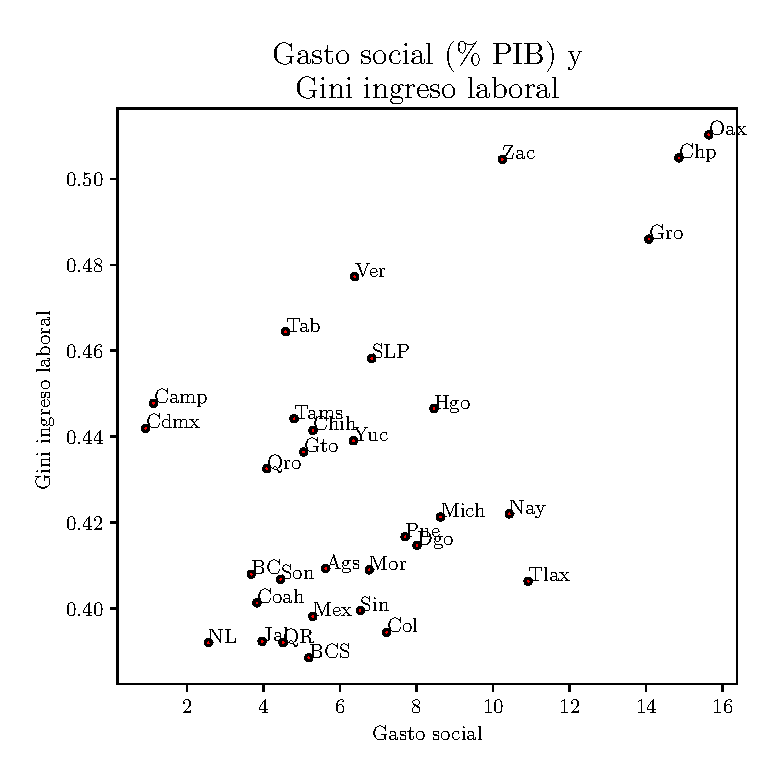
\includegraphics[width=.95\linewidth]{Graphs_tables_maps/Gs_Gini_ingreso_laboral.eps}
  %\caption{Gasto social e índice de Gini}
\end{subfigure}%
\begin{subfigure}{.5\textwidth}
  \centering
  \includegraphics[width=.95\linewidth]{Graphs_tables_maps/pca_Gini_ingreso_laboral.eps}
  %\caption{Índice de Gini y PCA}
\end{subfigure}
\begin{tiny}
\begin{spacing}{0}
\noindent Fuente: El índice de Gini fue elaborada basado en la Encuesta Nacional de Ingresos y Gastos de los Hogares 2016 elaborada por INEGI. El PCA (índice construido) fue construido basado en datos de la ENOE.
\end{spacing}
\end{tiny}
\end{figure}
%
Aunado a lo anterior, existe una relación positiva....

\begin{figure}[H]
\caption{Índice PCA1 y gasto social}
\begin{center}
\resizebox{4in}{!}{
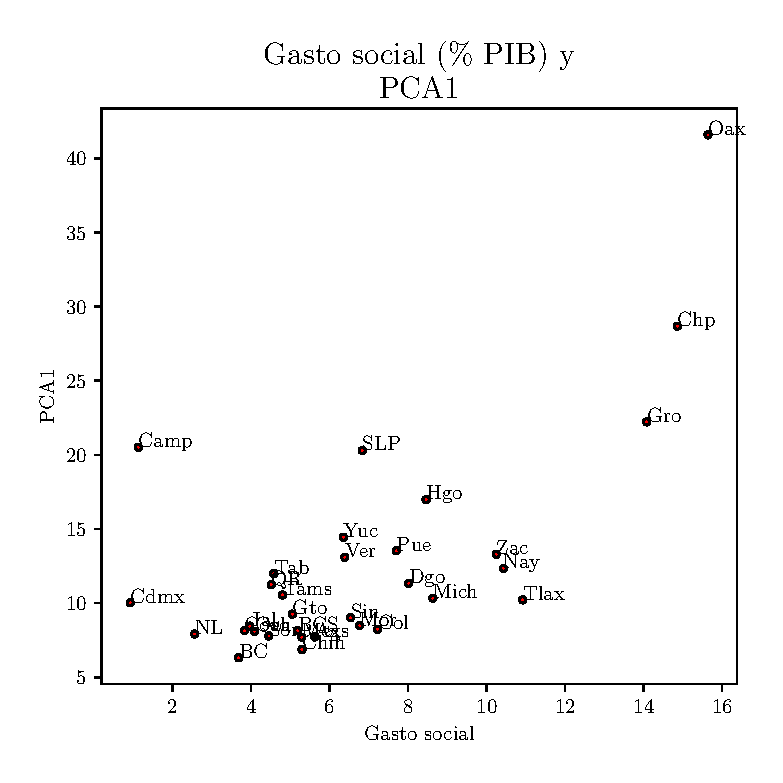
\includegraphics[width=\textwidth]{Graphs_tables_maps/pca.eps} } 
\end{center}
\begin{tiny}
\begin{spacing}{0}
\noindent \phantom{aaaaaaaaaaaaaaaaaaaaaaaaaaaa} Fuente: Elaboración propia.
\end{spacing}
\end{tiny}
\end{figure}




\subsection{Modelo}
	
En la presente subsección...
%
\begin{eqnarray}
D_{kj,t} &=&\beta_0 + \beta_1 D_{i,t-1} + \beta_2 a_{i,t} + \beta_3 Esc_{i,t}  \notag \\
 &&+ \beta_4 u_{i,t}  + \beta_5 d_{i,t}   + \beta_6 y_{i,t}  + \beta_7 y^2_{i,t}  + \beta_8 den_{i,t}  + v_{i} +  \mu_t  +\epsilon_{i,t} 
\end{eqnarray}
%
\section{Resultados del modelo}


A continuación se muestran los resultados. Se estiman MCO sin efectos y con efectos fijos por estado utilizando la ecuación 1. Para abordar el problema de endogeneidad, la ecuación 2 utiliza el estimador Arrellano-Bond instrumentando con los rezagos de 2 a 8 en niveles (colapsados) y el gasto electoral....


\begin{table}[H]
\begin{center}
\caption{Resultados estimación ecuación 1 por MCO sin efectos fijos}
\resizebox{6.5in}{!}{
\begin{tabular}{l*{22}{c}}
\hline\hline
                &\multicolumn{1}{c}{(1)}&\multicolumn{1}{c}{(2)}&\multicolumn{1}{c}{(3)}&\multicolumn{1}{c}{(4)}&\multicolumn{1}{c}{(5)}&\multicolumn{1}{c}{(6)}&\multicolumn{1}{c}{(7)}&\multicolumn{1}{c}{(8)}&\multicolumn{1}{c}{(9)}&\multicolumn{1}{c}{(10)}&\multicolumn{1}{c}{(11)}&\multicolumn{1}{c}{(12)}&\multicolumn{1}{c}{(13)}&\multicolumn{1}{c}{(14)}&\multicolumn{1}{c}{(15)}&\multicolumn{1}{c}{(16)}&\multicolumn{1}{c}{(17)}&\multicolumn{1}{c}{(18)}&\multicolumn{1}{c}{(19)}&\multicolumn{1}{c}{(20)}&\multicolumn{1}{c}{(21)}&\multicolumn{1}{c}{(22)}\\
                &\multicolumn{1}{c}{PCA1}&\multicolumn{1}{c}{P10P5}&\multicolumn{1}{c}{P25P5}&\multicolumn{1}{c}{P50P5}&\multicolumn{1}{c}{P75P5}&\multicolumn{1}{c}{P90P5}&\multicolumn{1}{c}{P95P5}&\multicolumn{1}{c}{P25P10}&\multicolumn{1}{c}{P50P10}&\multicolumn{1}{c}{P75P10}&\multicolumn{1}{c}{P90P10}&\multicolumn{1}{c}{P95P10}&\multicolumn{1}{c}{P50P25}&\multicolumn{1}{c}{P75P25}&\multicolumn{1}{c}{P90P25}&\multicolumn{1}{c}{P95P25}&\multicolumn{1}{c}{P75P50}&\multicolumn{1}{c}{P90P50}&\multicolumn{1}{c}{P95P50}&\multicolumn{1}{c}{P95P50}&\multicolumn{1}{c}{P95P50}&\multicolumn{1}{c}{P95P50}\\
                &     b/se        &     b/se        &     b/se        &     b/se        &     b/se        &     b/se        &     b/se        &     b/se        &     b/se        &     b/se        &     b/se        &     b/se        &     b/se        &     b/se        &     b/se        &     b/se        &     b/se        &     b/se        &     b/se        &     b/se        &     b/se        &     b/se        \\
\hline
Lag             &    0.841$^{***}$&    0.823$^{***}$&    0.890$^{***}$&    0.870$^{***}$&    0.859$^{***}$&    0.846$^{***}$&    0.834$^{***}$&    0.860$^{***}$&    0.849$^{***}$&    0.861$^{***}$&    0.861$^{***}$&    0.857$^{***}$&    0.873$^{***}$&    0.910$^{***}$&    0.917$^{***}$&    0.914$^{***}$&    0.814$^{***}$&    0.861$^{***}$&    0.864$^{***}$&    4.488$^{***}$&    2.074$^{***}$&    5.470$^{***}$\\
                &  (0.028)        &  (0.032)        &  (0.025)        &  (0.027)        &  (0.028)        &  (0.028)        &  (0.029)        &  (0.029)        &  (0.030)        &  (0.029)        &  (0.029)        &  (0.028)        &  (0.029)        &  (0.025)        &  (0.023)        &  (0.023)        &  (0.034)        &  (0.026)        &  (0.026)        &  (0.191)        &  (0.086)        &  (0.396)        \\
a               &    0.287$^{***}$&    0.005        &    0.024$^{*}$  &    0.089$^{***}$&    0.181$^{***}$&    0.349$^{***}$&    0.534$^{***}$&    0.010$^{*}$  &    0.048$^{***}$&    0.086$^{***}$&    0.156$^{***}$&    0.235$^{***}$&    0.011$^{***}$&    0.018$^{**}$ &    0.032$^{**}$ &    0.053$^{**}$ &    0.004$^{**}$ &    0.008$^{**}$ &    0.015$^{**}$ &    0.040$^{***}$&    0.048$^{***}$&    0.081$^{***}$\\
                &  (0.087)        &  (0.003)        &  (0.013)        &  (0.034)        &  (0.065)        &  (0.115)        &  (0.158)        &  (0.005)        &  (0.016)        &  (0.032)        &  (0.056)        &  (0.078)        &  (0.003)        &  (0.008)        &  (0.014)        &  (0.022)        &  (0.002)        &  (0.004)        &  (0.006)        &  (0.008)        &  (0.007)        &  (0.010)        \\
Escolaridad     &   -0.551        &    0.034$^{*}$  &    0.051        &   -0.037        &   -0.203        &   -0.490        &   -0.881        &    0.003        &   -0.120$^{*}$  &   -0.290$^{**}$ &   -0.556$^{**}$ &   -0.870$^{***}$&   -0.054$^{***}$&   -0.105$^{***}$&   -0.182$^{**}$ &   -0.289$^{***}$&   -0.022$^{***}$&   -0.039$^{**}$ &   -0.069$^{**}$ &   -0.241$^{***}$&   -0.297$^{***}$&   -0.442$^{***}$\\
                &  (0.347)        &  (0.017)        &  (0.061)        &  (0.142)        &  (0.266)        &  (0.464)        &  (0.636)        &  (0.024)        &  (0.063)        &  (0.125)        &  (0.227)        &  (0.317)        &  (0.016)        &  (0.037)        &  (0.070)        &  (0.106)        &  (0.008)        &  (0.018)        &  (0.030)        &  (0.037)        &  (0.036)        &  (0.047)        \\
u               &    0.033        &   -0.015$^{*}$  &   -0.018        &   -0.013        &   -0.013        &   -0.010        &    0.009        &    0.001        &    0.026        &    0.055        &    0.102        &    0.156        &    0.011$^{*}$  &    0.023        &    0.042        &    0.064        &   -0.001        &   -0.001        &   -0.000        &    0.037$^{**}$ &    0.020        &   -0.013        \\
                &  (0.168)        &  (0.008)        &  (0.030)        &  (0.071)        &  (0.132)        &  (0.228)        &  (0.312)        &  (0.012)        &  (0.030)        &  (0.057)        &  (0.102)        &  (0.141)        &  (0.007)        &  (0.015)        &  (0.029)        &  (0.045)        &  (0.003)        &  (0.008)        &  (0.014)        &  (0.018)        &  (0.017)        &  (0.023)        \\
d               &   -0.001        &    0.004        &    0.009        &    0.011        &    0.016        &    0.018        &    0.001        &    0.003        &   -0.001        &   -0.004        &   -0.013        &   -0.033        &   -0.003        &   -0.004        &   -0.007        &   -0.016        &   -0.000        &   -0.001        &   -0.004        &   -0.004        &   -0.012$^{**}$ &   -0.028$^{***}$\\
                &  (0.052)        &  (0.003)        &  (0.010)        &  (0.022)        &  (0.041)        &  (0.070)        &  (0.096)        &  (0.004)        &  (0.009)        &  (0.018)        &  (0.031)        &  (0.044)        &  (0.002)        &  (0.005)        &  (0.009)        &  (0.014)        &  (0.001)        &  (0.002)        &  (0.004)        &  (0.005)        &  (0.005)        &  (0.007)        \\
y               &    0.016$^{***}$&    0.000        &    0.001        &    0.005$^{*}$  &    0.010$^{**}$ &    0.020$^{**}$ &    0.030$^{***}$&    0.000        &    0.002$^{**}$ &    0.005$^{**}$ &    0.009$^{**}$ &    0.014$^{**}$ &    0.001$^{**}$ &    0.001$^{**}$ &    0.002$^{**}$ &    0.004$^{**}$ &    0.000$^{***}$&    0.001$^{**}$ &    0.002$^{***}$&    0.004$^{***}$&    0.003$^{***}$&    0.005$^{***}$\\
                &  (0.006)        &  (0.000)        &  (0.001)        &  (0.002)        &  (0.005)        &  (0.008)        &  (0.011)        &  (0.000)        &  (0.001)        &  (0.002)        &  (0.004)        &  (0.006)        &  (0.000)        &  (0.001)        &  (0.001)        &  (0.002)        &  (0.000)        &  (0.000)        &  (0.001)        &  (0.001)        &  (0.001)        &  (0.001)        \\
$ y^2 $         &   -0.000$^{**}$ &   -0.000        &   -0.000        &   -0.000        &   -0.000$^{*}$  &   -0.000$^{**}$ &   -0.000$^{**}$ &   -0.000        &   -0.000        &   -0.000$^{*}$  &   -0.000$^{*}$  &   -0.000$^{**}$ &   -0.000$^{**}$ &   -0.000$^{*}$  &   -0.000$^{*}$  &   -0.000$^{*}$  &   -0.000$^{**}$ &   -0.000$^{**}$ &   -0.000$^{**}$ &   -0.000$^{***}$&   -0.000$^{***}$&   -0.000$^{***}$\\
                &  (0.000)        &  (0.000)        &  (0.000)        &  (0.000)        &  (0.000)        &  (0.000)        &  (0.000)        &  (0.000)        &  (0.000)        &  (0.000)        &  (0.000)        &  (0.000)        &  (0.000)        &  (0.000)        &  (0.000)        &  (0.000)        &  (0.000)        &  (0.000)        &  (0.000)        &  (0.000)        &  (0.000)        &  (0.000)        \\
den             &    0.000        &   -0.000        &    0.000        &    0.000        &    0.000        &    0.000        &    0.000        &    0.000        &    0.000        &    0.000$^{*}$  &    0.000$^{*}$  &    0.000$^{*}$  &    0.000$^{*}$  &    0.000$^{*}$  &    0.000        &    0.000        &    0.000$^{***}$&    0.000$^{**}$ &    0.000$^{*}$  &    0.000$^{***}$&    0.000$^{***}$&    0.000$^{***}$\\
                &  (0.000)        &  (0.000)        &  (0.000)        &  (0.000)        &  (0.000)        &  (0.000)        &  (0.000)        &  (0.000)        &  (0.000)        &  (0.000)        &  (0.000)        &  (0.000)        &  (0.000)        &  (0.000)        &  (0.000)        &  (0.000)        &  (0.000)        &  (0.000)        &  (0.000)        &  (0.000)        &  (0.000)        &  (0.000)        \\
Constante       &    2.212        &   -0.277        &   -0.727        &   -0.798        &   -0.507        &    0.228        &    2.613        &   -0.076        &    0.824        &    2.030        &    4.880        &    8.162$^{*}$  &    0.646$^{***}$&    1.025$^{**}$ &    1.611$^{*}$  &    2.654$^{*}$  &    0.438$^{***}$&    0.546$^{**}$ &    0.877$^{**}$ &   -2.195$^{***}$&    1.480$^{***}$&    0.282        \\
                &  (4.699)        &  (0.232)        &  (0.883)        &  (1.987)        &  (3.673)        &  (6.359)        &  (8.687)        &  (0.329)        &  (0.852)        &  (1.634)        &  (3.042)        &  (4.235)        &  (0.216)        &  (0.488)        &  (0.922)        &  (1.389)        &  (0.126)        &  (0.260)        &  (0.429)        &  (0.632)        &  (0.537)        &  (0.826)        \\
\hline
N               &  288.000        &  288.000        &  288.000        &  288.000        &  288.000        &  288.000        &  288.000        &  288.000        &  288.000        &  288.000        &  288.000        &  288.000        &  288.000        &  288.000        &  288.000        &  288.000        &  288.000        &  288.000        &  288.000        &  288.000        &  288.000        &  288.000        \\
r2              &    0.940        &    0.834        &    0.921        &    0.933        &    0.937        &    0.935        &    0.935        &    0.905        &    0.939        &    0.949        &    0.949        &    0.950        &    0.943        &    0.955        &    0.957        &    0.954        &    0.911        &    0.930        &    0.923        &    0.875        &    0.878        &    0.776        \\
\hline\hline
\multicolumn{23}{l}{\footnotesize $^{*}$ \(p<0.10\), $^{**}$ \(p<0.05\), $^{***}$ \(p<0.01\)}\\
\end{tabular}
}
\end{center}
\begin{tiny}
Nota: Se generan los estimadores ponderados por la población por estado en $t$ y se presentan errores por clusters por estado.
\end{tiny}
\end{table}

....


\subsection{Modelo de equilibrio}

....

\section{Conclusiones y consideraciones finales}

....





\pagebreak

\addcontentsline{toc}{section}{Bibliografía}
\renewcommand{\refname}{Bibliografía}
\bibliographystyle{apalike-es}

\spacing{1}
\bibliography{mybib}


\newpage


\newpage
\spacing{1}
\appendix    

\section*{Anexos} 
\addcontentsline{toc}{section}{Anexo}
Anexo....





\end{document}
